\chapter{Database Design}

\section{Working}
The system is designed to work in the following way:
\begin{itemize}
    \item The user connects their smartphone to the Rokers system via the internet.
    \item The user opens the Rokers app on their smartphone and logs in to their Spotify account.
    \item The app fetches music information from Spotify API and stores it in a MySQL database.
    \item The user can then select and play music through the inbuilt speaker.
The system keeps a record of the music playback in the MySQL database.
\end{itemize}





\section{Entities, Attributes and Relationships}
The database, called rokers, will have five tables, songs, albums, artits, playlists, songArtist. Each will hold information about songs and the artistis and other important details. The two
tables will be linked through a foreign key. The student table has the following fields:\\

\section{ER Schema}
\begin{figure}[H]
\centering
\caption{Entity Relationship Diagram}
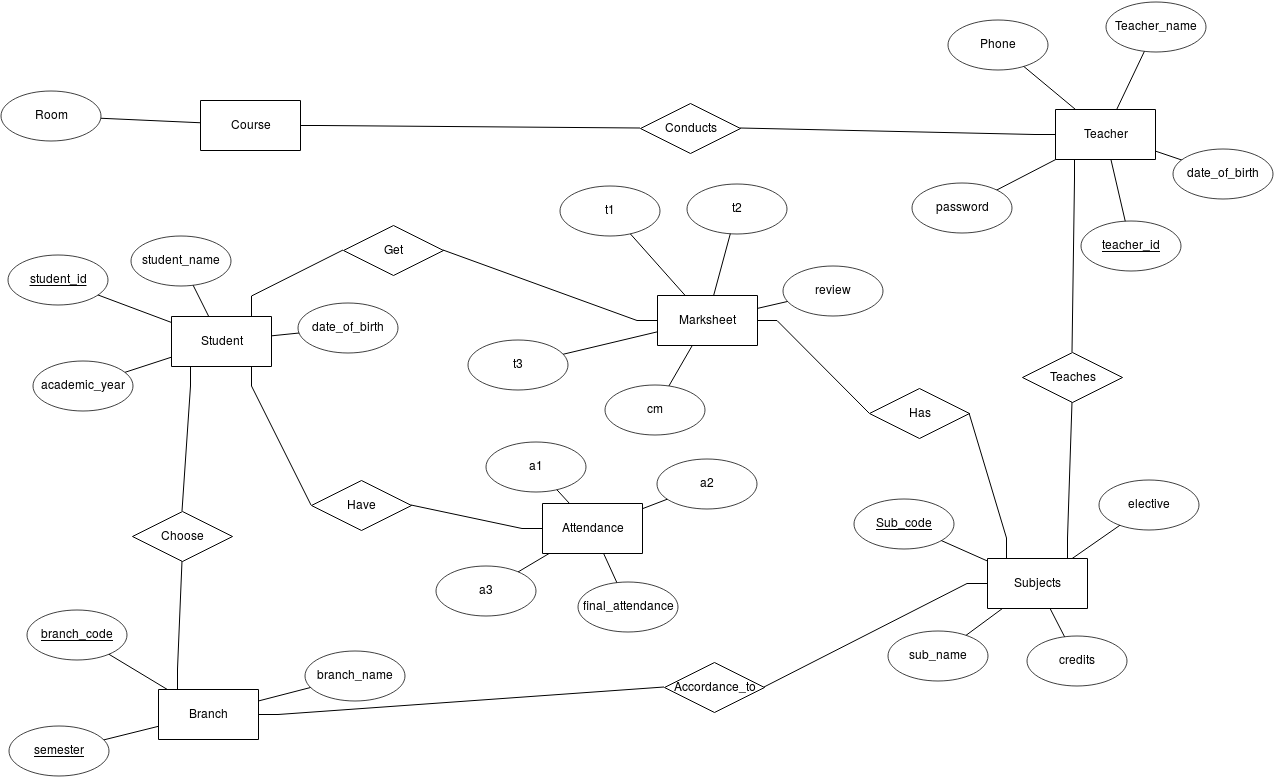
\includegraphics[width=\textwidth,height=\textheight,keepaspectratio]{./erd.png}
\\[0.2in]
\label{fig:Entitiy Relationship Diagram}
\end{figure}

\pagebreak
\thispagestyle{fancy}

\section{Schema Diagram}
\begin{figure}[H]
\centering
\caption{Relational Schema}
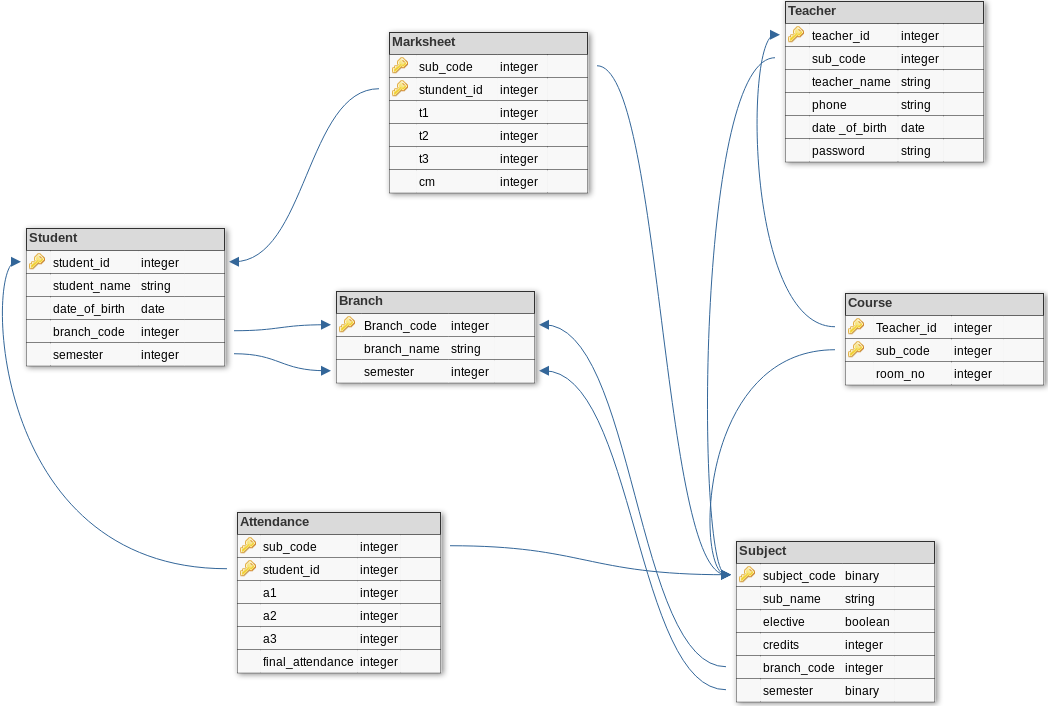
\includegraphics[scale=.5]{./schema.png}
\\[0.2in]
\label{fig:Relational Schema}
\end{figure}

\thispagestyle{fancy}